\newpage
\texHeader

{\bf \Large 2 \hspace{0.5cm}Static semantics}

\subsection[A Concrete Defintion (Textual)]{A Concrete Definition; Developing with MOSL}
\label{sec:staticConcrete}

\begin{itemize}

\item[$\blacktriangleright$] \hypertarget{static tex}{Begin a} new metamodel project from eclipse by navigating to the \texttt{New Metamodel} button on the toolbar (fig.~\ref{fig:new_project}). In the dialog that appears, enter \texttt{LeitnersLearningBox} as the project name, and select \texttt{Textual (MOSL)}.

\begin{figure}[htbp]
	\centering
  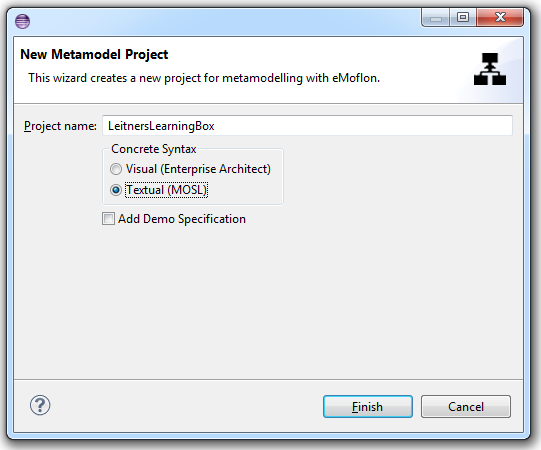
\includegraphics[width=0.7\textwidth]{eclipse_newMetamodelTextPlain}
	\caption{Create a new concrete metamodeling project}
	\label{fig:new_project}
\end{figure}

\item[$\blacktriangleright$] Expand the project as deep as it goes (fig.~\ref{fig:expanded_folders}). Your \texttt{Package explorer} will look different depending on whether or not you completed the Demo in \texttt{Part I}. Don't be concerned though - those files no longer matter. This handbook has removed them from the screenshots, but we recommend you keep them around for reference.

\begin{figure}[htbp]
	\centering
  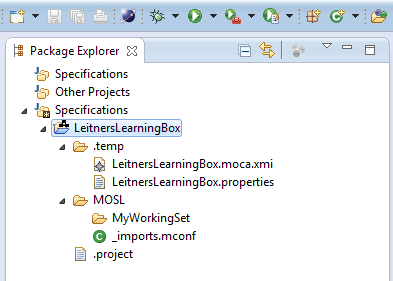
\includegraphics[width=0.7\textwidth]{eclipse_foldersExpanded}
	\caption{Expanded project files}
	\label{fig:expanded_folders}
\end{figure} 

\item[$\blacktriangleright$] You can see three folders - \texttt{.temp}, \texttt{MOSL}, and \texttt{MyWorkingSet} - as well as a global \texttt{\_imports.mconf} file. To summarize, \texttt{MOSL} contains the \texttt{MyWorkingSet} workspace, which in turn will contain a folder for each project built with eMoflon. For detailed information on the file structure and set up, review \texttt{Part I} of the handbook.

\item[$\blacktriangleright$] Right click on \texttt{MyWorkingSet} and create a new folder. In the dialog that appears, name it \texttt{LearningBoxLanguage}. This is now the container for all your modeling files!

\pagebreak

\item[$\blacktriangleright$] Following the same logic that's found in the Object Oriented Paradigm where ``everything is an object,'' in metamodelling, everything is a model. If everything is a model, a metamodel that defines (at least a part of) a language must be a model itself. This means that it conforms to some meta-metamodel which defines a (meta)modelling language or meta-language. For metamodelling with eMoflon, we support Ecore as a modelling language and it defines types like EClass and EReference, which we will be using to specify our metamodels. Other modelling languages include MOF, UML and Kermeta. % This is something no-one wants to read. Re-word??

\item[$\blacktriangleright$] Right click on \texttt{LearningBoxLanguage} and create your first eclass model by going to ``New/EClass.'' Name it \texttt{Box}.

\item[$\blacktriangleright$] The class editor should have automatically appeared. Currently, it's empty; Lets add the first two attributes of our program, \texttt{name} and \texttt{stringRep}. Both are \texttt{EString} types (fig~\ref{fig:boxDeclaration}).

\begin{figure}[htbp]
	\centering
  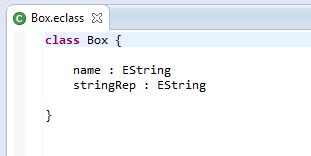
\includegraphics[width=0.5\textwidth]{eclipse_classBoxDeclaration}
	\caption{Newly created box class}
	\label{fig:boxDeclaration}
\end{figure} 

\item[$\blacktriangleright$] Create two more classes in your model the same way, called \texttt{Partition} and \texttt{Card}. 

\item[$\blacktriangleright$] In \texttt{Partition}, add two \texttt{EInt} datatypes, \texttt{index} and \texttt{partitionSize}. 

\item[$\blacktriangleright$] In \texttt{Card}, create three \texttt{EString}s, \texttt{back}, \texttt{face} , and \texttt{partitionHistory}.

\item[$\blacktriangleright$] If you've done everything correctly, the key spaces in your workspace should now resemble Figure~\ref{fig:workspaceClassAttributes}.

\begin{figure}[htbp]
	\centering
  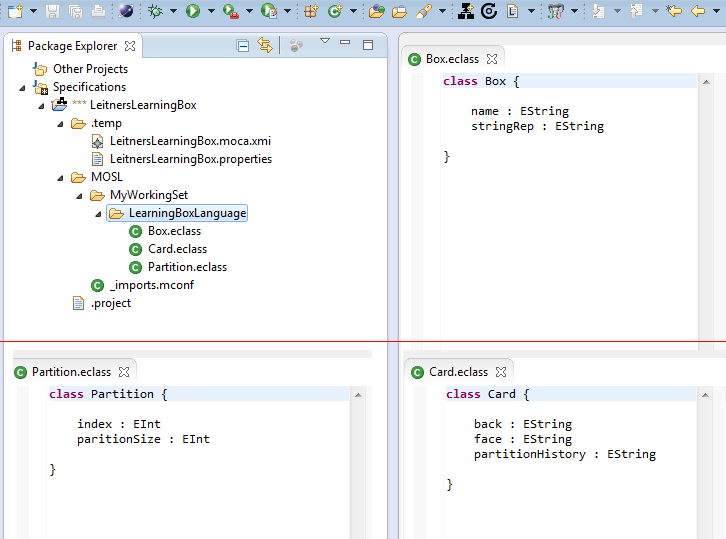
\includegraphics[width=0.9\textwidth]{eclipse_workspaceClassesAttributes}
	\caption{Declaration of classes and attributes}
	\label{fig:workspaceClassAttributes}
\end{figure} 

\item[$\blacktriangleright$] Now lets add some references. MOSL supports two reference types, the \emph{contained reference} and the \emph{simple reference}, and both automatically update the other element involved in the reference automatically, which means you only have to declare a direction once. Neat, huh?

\item[$\blacktriangleright$] Activate the \texttt{Card} model and add a simple reference named \texttt{cardContainer} with a multiplicity of zero to one, of type \texttt{Partition} (fig.~\ref{fig:cardReference}). This means that a single card can belong to a maximum of 1 partition.

\begin{figure}[htbp]
	\centering
  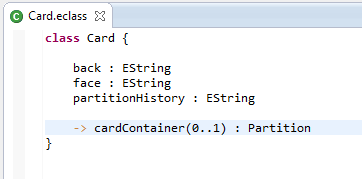
\includegraphics[width=0.5\textwidth]{eclipse_cardReference}
	\caption{Creating a \emph{simple reference} in Card}
	\label{fig:cardReference}
\end{figure} 

\item[$\blacktriangleright$] Now add a \emph{container reference} to \texttt{Partition}. Name it \texttt{card}, and allow it to hold an unlimited amount of cards.

\item[$\blacktriangleright$] Congratulations, you just built your first \emph{Bidirectional EReference}! In essence, you have now set up a relation that allows a potentially infinite amount of item \texttt{card} to be stored in a partition, and restricts the \texttt{containedCard} to only \emph{one} partition.

\item[$\blacktriangleright$] Now, lets create another bidirectional association between \texttt{Partition} and \texttt{Box}. If you think about it, it's really not all that different than the relation between \texttt{Partition} and \texttt{Card}. In fact, it's not different at all! A \texttt{Box} should be able to hold an unlimited amount of partitions, but a \texttt{Partition} should only be allowed to belong to zero or one boxes. Name the two new relations \texttt{containedPartition}, and \texttt{box}. 

\item[$\blacktriangleright$] Your classes should now closely resemble figure~\ref{fig:allReferences}


\begin{figure}[htbp]
	\centering
  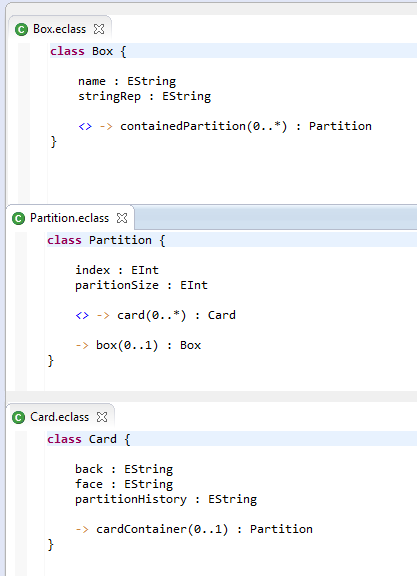
\includegraphics[width=0.5\textwidth]{eclipse_workspaceReferences}
	\caption{Each class with the appropriate references}
	\label{fig:allReferences}
\end{figure} 


\item[$\blacktriangleright$] The next thing we need to do is set up two relations between \texttt{Partition} and itself, so it can able shift between the previous and next partitions. Create two new simple references, named \texttt{previous}, and \texttt{next}. Allow them to have a maximum of 1 link each.

\item[$\blacktriangleright$] If you've done everything correctly, your \texttt{Partition} class should now resemble figure~\ref{fig:partitionReferences}
section~\ref{sec:staticAbstract}

\begin{figure}[htbp]
	\centering
  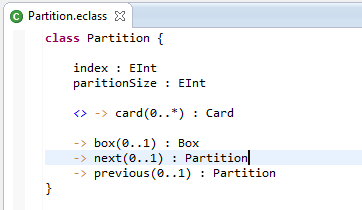
\includegraphics[width=0.5\textwidth]{eclipse_partitionReferences}
	\caption{All references in Partition}
	\label{fig:partitionReferences}
\end{figure} 

\item[$\blacktriangleright$] All of our references are now set up! To see how figures \ref{fig:allReferences} and \ref{fig:partitionReferences} are depicted visually, check out figure~\ref{fig:ereferences_all} in section~\ref{sec:staticAbstract}.

\item[$\blacktriangleright$] You're almost done setting up your static model! The last thing we need to do is to make the program \emph{do} something. After all, what good is a program that only stores attributes and references?

\item[$\blacktriangleright$] Lets continue with the \texttt{Partition} class. We want the partitions to be able to do three things - check the answer of a flashcard with a guess, remove a card if that answer is correct, and empty the partition of all cards to reset. Start with the \texttt{empty} method - it won't need any paramters, and it doesn't need to return anything. Declare a parameter-free \emph{void} function\footnote{If you're having difficulty remembering the syntax for MOSL, feel free to review \mbox{\texttt{Part I}}}.

\item[$\blacktriangleright$] Unfortunately, in our MOSL language, a function declaration is not enough to fully establish it. If you remember from \texttt{Part I}, each function needs its own folder within the workspace to store the dynamic action, or \emph{pattern}. Select the \texttt{LearningBoxLanguage} folder, and create a new folder named \texttt{\_patterns}. Within this space, create another folder with the same name as your function.

\item[$\blacktriangleright$] If you did this step correctly, your project explorer should now resemble figure~\ref{fig:emptyFolder}.

%% =========================================== REDO REDO =================================================
\begin{figure}[htbp]
	\centering
  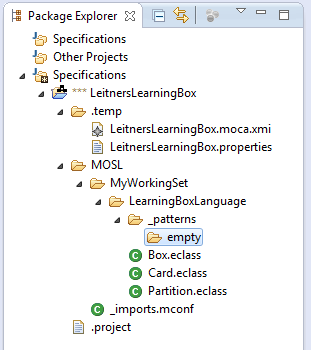
\includegraphics[width=0.5\textwidth]{eclipse_projectExplorerEmptyFunction}
	\caption{The \texttt{empty} method folder {\bf incorrect image: update}}
	\label{fig:emptyFolder}
\end{figure} 
%% =========================================== REDO REDO =================================================

\item[$\blacktriangleright$] Create two more functions in \texttt{Partition} the same way. We'll need a \texttt{removeCard} method that accepts and returns a \texttt{Card}, as well as a EBoolean \texttt{check} method that accepts a \texttt{Card} and an \texttt{EString} guess.

\item[$\blacktriangleright$] Your partition class should now resemble figure~\ref{fig:partitionComplete}.

\begin{figure}[htbp]
	\centering
  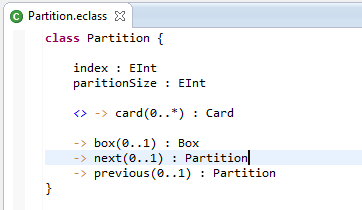
\includegraphics[width=0.5\textwidth]{eclipse_partitionReferences}
	\caption{The completed \texttt{Partition} class}
	\label{fig:partitionComplete}
\end{figure}

\item[$\blacktriangleright$] What needs to be done in the \texttt{Card} class? Well, in order to check the card, we'll need to be able to look at the flip side. We'll also need to print whatever is on the current side. Create two void functions, \texttt{invert} and \texttt{printCard}.

\item[$\blacktriangleright$] Finally, what do we need to do with the largest object in our model, the overall \texttt{Box}? In summary, we want to allow \texttt{Box} to:

\begin{description}
	{\small
  \item[\texttt{determineNextSize():EInt }] find out how big the upcoming partition is
  \item[\texttt{grow():void}] increase in size to allow more partitions
  \item[\texttt{toString():EString}] let user see all partitions in the current box
  \item[\texttt{addToStringRep(card:Card):void}] not sure yet
  }
\end{description}


\item[$\blacktriangleright$] Your workspace should now resemble figure~\ref{fig:workspaceMethods}. Be sure to examine the \texttt{Package Explorer} to make sure you've set up the folders correctly! This will imperative in the next part, when we're modeling dynamic semantics using Story Driven Modeling (SDMs).

\begin{figure}[htbp]
	\centering
  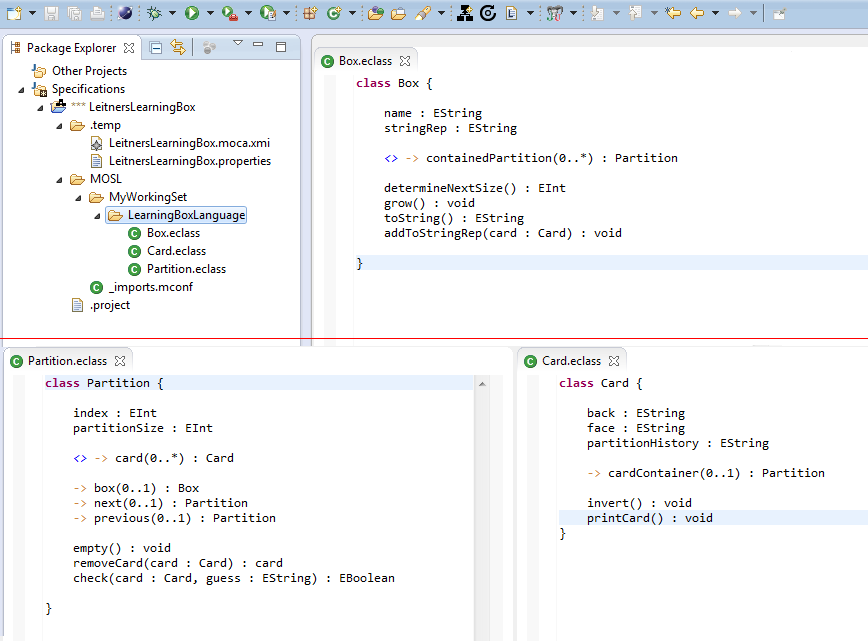
\includegraphics[width=0.9\textwidth]{eclipse_workspaceMethods}
	\caption{Each class and their methods}
	\label{fig:workspaceMethods}
\end{figure}


\item[$\blacktriangleright$] Congratulations! You've \emph{almost} completeley modeled Leitner's Learning Box using a concrete, textual syntax! To see how this looks in a visual class diagram, check out figure~\ref{fig:metamodel_complete} from section~\ref{sec:staticAbstract}.

\item[$\blacktriangleright$]The very last thing we need to do now is build it and generate the required \texttt{.genmodel} and \texttt{.ecore} files. 

\item[$\blacktriangleright$] Beside the \texttt{New Metamodel} button on the toolbar, you'll notice that there is a button that looks like a circular arrow which offers to ``Build (without cleaning).'' %Explain this here?
If you've done everything correctly, a new \texttt{MyWorkingSet} node should have appeared should have appeared. Expand it to see a metamodel folder named \texttt{LearningBoxLanguage}. 

\item[$\blacktriangleright$] Examine the \texttt{gen} folder. % (why? check VIS)

\item[$\blacktriangleright$] Finally, you can see that your two metamodels have been created and placed in the \texttt{model} folder. Together, they form everything the EMF needs to generate your program.

\fancyfoot[R]{ $\triangleright$ \hyperlink{validation tex}{Next step} }

\item[$\blacktriangleright$] You're all done! We encourage you to review section~\ref{sec:staticAbstract} and observe how this same project is crafted using visual tools. Compare the differences between modeling the three classes in a seprate, abstract program, and then building them, versus modeling and building all within eclipse. Which do you find easier to work with?

\end{itemize}